\documentclass{article}
\usepackage[table,xcdraw]{xcolor}
\usepackage{graphicx}
\usepackage{listings}
\usepackage{hyperref}
\usepackage{pdfpages}
\usepackage{csvsimple}
\usepackage{float}
\makeatletter
\newcommand\urlfootnote@[1]{\footnote{\url@{#1}}}
\DeclareRobustCommand{\urlfootnote}{\hyper@normalise\urlfootnote@}
\makeatother

\begin{document}
\title{Neural Networks Assignment 1}
\author{Group 35}
\maketitle
\lstset{
  basicstyle=\ttfamily,
  keywordstyle=\bfseries,
  language=Java,
  frame=single,
  aboveskip=11pt,
  belowskip=11pt,
  breaklines=true,
  breakatwhitespace=false,
  showspaces=false,
  showstringspaces=false,
  numbers=left,
  stepnumber=1,    
  firstnumber=1,
  numberfirstline=true
}
\section{Excercise 1: Image Distance}
\label{a1}

After running the program we received the following cloud distances for the digits 0 - 9 (see Table \ref{table:distances}):

% Please add the following required packages to your document preamble:
% \usepackage[table,xcdraw]{xcolor}
% If you use beamer only pass "xcolor=table" option, i.e. \documentclass[xcolor=table]{beamer}
\begin{table}[H]
	\centering
	\label{my-label}
	\begin{tabular}{lllllllllll}
		                      & 0                                                 & 1                                                 & 2                                                 & 3                                                 & 4                                                 & 5                                                 & 6                                                 & 7                                                 & 8                                                 & 9                                                 \\ \cline{2-11} 
		\multicolumn{1}{l|}{0} & \multicolumn{1}{l|}{\cellcolor[HTML]{C0C0C0}0.00} & \multicolumn{1}{l|}{14.45}                        & \multicolumn{1}{l|}{9.33}                         & \multicolumn{1}{l|}{9.14}                         & \multicolumn{1}{l|}{10.77}                        & \multicolumn{1}{l|}{7.52}                         & \multicolumn{1}{l|}{8.15}                         & \multicolumn{1}{l|}{11.86}                        & \multicolumn{1}{l|}{9.91}                         & \multicolumn{1}{l|}{11.49}                        \\ \cline{2-11} 
		\multicolumn{1}{l|}{1} & \multicolumn{1}{l|}{14.45}                        & \multicolumn{1}{l|}{\cellcolor[HTML]{C0C0C0}0.00} & \multicolumn{1}{l|}{10.13}                        & \multicolumn{1}{l|}{11.73}                        & \multicolumn{1}{l|}{10.17}                        & \multicolumn{1}{l|}{11.12}                        & \multicolumn{1}{l|}{10.61}                        & \multicolumn{1}{l|}{10.74}                        & \multicolumn{1}{l|}{10.09}                        & \multicolumn{1}{l|}{9.93}                         \\ \cline{2-11} 
		\multicolumn{1}{l|}{2} & \multicolumn{1}{l|}{9.33}                         & \multicolumn{1}{l|}{10.13}                        & \multicolumn{1}{l|}{\cellcolor[HTML]{C0C0C0}0.00} & \multicolumn{1}{l|}{8.18}                         & \multicolumn{1}{l|}{7.93}                         & \multicolumn{1}{l|}{7.91}                         & \multicolumn{1}{l|}{7.33}                         & \multicolumn{1}{l|}{8.87}                         & \multicolumn{1}{l|}{7.08}                         & \multicolumn{1}{l|}{8.89}                         \\ \cline{2-11} 
		\multicolumn{1}{l|}{3} & \multicolumn{1}{l|}{9.14}                         & \multicolumn{1}{l|}{11.73}                        & \multicolumn{1}{l|}{8.18}                         & \multicolumn{1}{l|}{\cellcolor[HTML]{C0C0C0}0.00} & \multicolumn{1}{l|}{9.09}                         & \multicolumn{1}{l|}{6.12}                         & \multicolumn{1}{l|}{9.30}                         & \multicolumn{1}{l|}{8.92}                         & \multicolumn{1}{l|}{7.02}                         & \multicolumn{1}{l|}{8.35}                         \\ \cline{2-11} 
		\multicolumn{1}{l|}{4} & \multicolumn{1}{l|}{10.77}                        & \multicolumn{1}{l|}{10.17}                        & \multicolumn{1}{l|}{7.93}                         & \multicolumn{1}{l|}{9.09}                         & \multicolumn{1}{l|}{\cellcolor[HTML]{C0C0C0}0.00} & \multicolumn{1}{l|}{8.00}                         & \multicolumn{1}{l|}{8.78}                         & \multicolumn{1}{l|}{7.58}                         & \multicolumn{1}{l|}{7.38}                         & \multicolumn{1}{l|}{6.01}                         \\ \cline{2-11} 
		\multicolumn{1}{l|}{5} & \multicolumn{1}{l|}{7.52}                         & \multicolumn{1}{l|}{11.12}                        & \multicolumn{1}{l|}{7.91}                         & \multicolumn{1}{l|}{6.12}                         & \multicolumn{1}{l|}{8.00}                         & \multicolumn{1}{l|}{\cellcolor[HTML]{C0C0C0}0.00} & \multicolumn{1}{l|}{6.70}                         & \multicolumn{1}{l|}{9.21}                         & \multicolumn{1}{l|}{6.97}                         & \multicolumn{1}{l|}{8.26}                         \\ \cline{2-11} 
		\multicolumn{1}{l|}{6} & \multicolumn{1}{l|}{8.15}                         & \multicolumn{1}{l|}{10.61}                        & \multicolumn{1}{l|}{7.33}                         & \multicolumn{1}{l|}{9.30}                         & \multicolumn{1}{l|}{8.78}                         & \multicolumn{1}{l|}{6.70}                         & \multicolumn{1}{l|}{\cellcolor[HTML]{C0C0C0}0.00} & \multicolumn{1}{l|}{10.89}                        & \multicolumn{1}{l|}{8.59}                         & \multicolumn{1}{l|}{10.44}                        \\ \cline{2-11} 
		\multicolumn{1}{l|}{7} & \multicolumn{1}{l|}{11.86}                        & \multicolumn{1}{l|}{10.74}                        & \multicolumn{1}{l|}{8.87}                         & \multicolumn{1}{l|}{8.92}                         & \multicolumn{1}{l|}{7.58}                         & \multicolumn{1}{l|}{9.21}                         & \multicolumn{1}{l|}{10.89}                        & \multicolumn{1}{l|}{\cellcolor[HTML]{C0C0C0}0.00} & \multicolumn{1}{l|}{8.47}                         & \multicolumn{1}{l|}{5.43}                         \\ \cline{2-11} 
		\multicolumn{1}{l|}{8} & \multicolumn{1}{l|}{9.91}                         & \multicolumn{1}{l|}{10.09}                        & \multicolumn{1}{l|}{7.08}                         & \multicolumn{1}{l|}{7.02}                         & \multicolumn{1}{l|}{7.38}                         & \multicolumn{1}{l|}{6.97}                         & \multicolumn{1}{l|}{8.59}                         & \multicolumn{1}{l|}{8.47}                         & \multicolumn{1}{l|}{\cellcolor[HTML]{C0C0C0}0.00} & \multicolumn{1}{l|}{6.40}                         \\ \cline{2-11} 
		\multicolumn{1}{l|}{9} & \multicolumn{1}{l|}{11.49}                        & \multicolumn{1}{l|}{9.93}                         & \multicolumn{1}{l|}{8.89}                         & \multicolumn{1}{l|}{8.35}                         & \multicolumn{1}{l|}{6.01}                         & \multicolumn{1}{l|}{8.26}                         & \multicolumn{1}{l|}{10.44}                        & \multicolumn{1}{l|}{5.43}                         & \multicolumn{1}{l|}{6.40}                         & \multicolumn{1}{l|}{\cellcolor[HTML]{C0C0C0}0.00} \\ \cline{2-11} 	
	\end{tabular}
	\caption{Cloud distances for the digit 0 - 9}
	\label{table:distances}
\end{table}

When looking at the cloud distances, we can assume that the most difficult digits to separate from each other are: \[ 7 \leftrightarrow 9; 4 \leftrightarrow 9; 3 \leftrightarrow 5; 9 \leftrightarrow 8\]
 
This can be concluded by looking at the distance values of these digits. The lowest distance and hence the most similar classes we found were 5.43, 6.01, 6.12 and 6.4.
These are the distances for the digits mentioned above.
This does make sense given that a 9 can be, if written by hand, sometimes hard to distinguish from a 7, 4 or 5.

\newpage
\section{Excercise 2}
\subsection{Confusion Matrix Training and Test Set}
The confusion matrix for the training set can be found in Figure \ref{fig:cftrain} and the confusion matrix for the test set can be found in Figure \ref{fig:cftest}.
Each element shows the rate of correct classifications,hence a value above 1 is not possible.
The y-axis indicates the recognized number, while the x-axis indicates the actual number of a sample.
For example: A value of 0.7 expresses, that the recognized number was identified as the actual number in 70\% of the test cases.

For the training set the numbers 4 and 5 are most difficult to classify. The only number with no misclassification is 1. This is quite surprising given that 1 and 7 sometimes look quite alike.

For the test set (Figure \ref{fig:cftest}) the number 2 is most difficult to classify. Followed by 0, 8, 9, 7 and 3. Also here we have almost full accuracy for the digit 1 (99\%).




\begin{figure}[H]
\centering
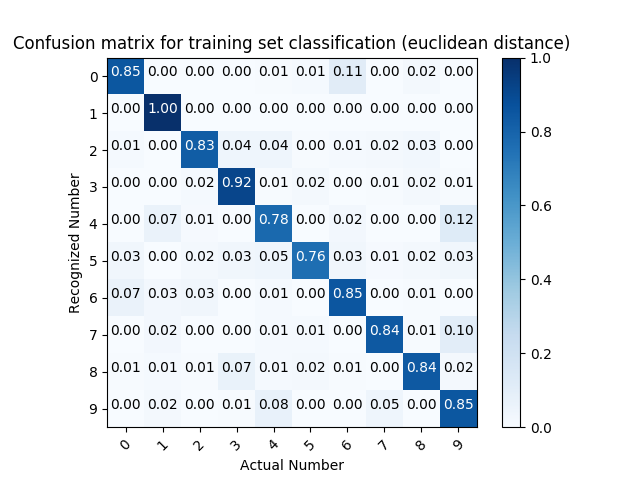
\includegraphics[width=0.9\linewidth]{img/2/Training-Set-CM-euclidean.png}
\caption{Confusion Matrix for the training set}
\label{fig:cftrain}
\end{figure}
\begin{figure}[H]
\centering
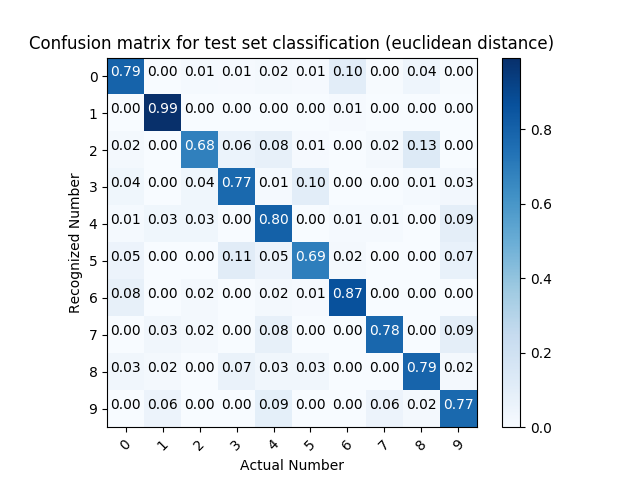
\includegraphics[width=0.9\linewidth]{img/2/Test-Set-CM-euclidean.png}
\caption{Confusion Matrix for the test set}
\label{fig:cftest}
\end{figure}



\subsection{Comparison to expectations from A1}
%How do the results compare to the observations you’ve made in Step 1? How would you explain it?%
When comparing our findings with the expectations build up in Excercise 1 (see Section \ref{a1}) the occurred misclassifications are quite different.
If we look at the confusion matrix of the training set our expectations are mostly met. This is because here the  most often misclassified numbers are 4 $\rightarrow$ 9, 7 $\rightarrow$ 9 and 4 $\rightarrow$ 6.
For the test set however this does not prove to be true. Here the most often misclassified numbers are 2 $\rightarrow$ 8, 0 $\rightarrow$ 6 and 9 $\rightarrow$ 4.

This difference could be explained by the amount of actual sample numbers per digit in the classified set.
But more likely the phenomena of \emph{overfitting} plays a huge role in the differing results.

\subsection{Evaluating different performance measures}
%Which distance measure provides best results (on the test set)?%
In order to determine which distance provider faired out the best, we applied each of them to the test set and measured the amount of correctly classified occurrences.

Results for the test set (sorted by best first):
\begin{itemize}
\item Euclidian (L2): 80.4\% $\rightarrow$ 804 / 1000 correctly classified
\item Cosine 79.9\% $\rightarrow$ 799 / 1000 correctly classified
\item Manhattan (Cityblock, L1): 72.1\% $\rightarrow$ 721 / 1000 correctly classified
\end{itemize}

As you can obviously tell, the euclidian distance turns out to be best (only for this example of course).

\section{Exercise 3: Bayesian Classification}
For this exercise we implemented the bayer rule classifier according to the lecture. In this section we will first discuss the chosen feature and digits.
After that we will take a look at the achieved results.

\subsection{Feature \& Test Digits}
We will be comparing the digits \textbf{7} and \textbf{8}.
To compare these two numbers we will use the ratio between the upper and the lower half of the image. We decided to use this feature because it is dead simple to extract, but should be different enough to distinguish between a 7 and an 8. While the ratio for the digit 8 should be around 1, the ratio for the digit 7 should be above 1.


%Implement your feature, apply it to the training data, discretize it and create corresponding histograms.%
\subsection{Histogram}
The histogram for the digits 7 and 8 with our feature applied can be seen in Figure \ref{fig:histogram}.
As you can see, the overlapping area is quite small. Only between around 1.3 to 1.5 it might be difficult to separate the two digits.

\begin{figure}[H]
	\centering
	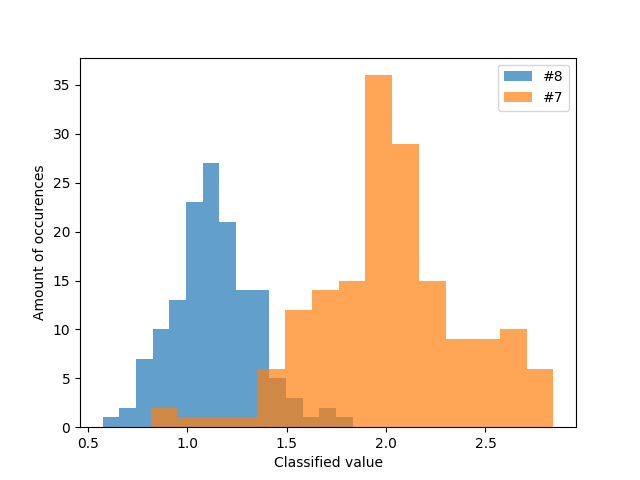
\includegraphics[width=0.9\linewidth]{img/3/histogram.png}
	\caption{Histogram for identifying digit 7 and digit 8 based on our selected feature.}
	\label{fig:histogram}
\end{figure}

\subsection{Results}
We achieved an accuracy of 92.95\% on the test set. Out of 156 samples 145 turns out to be classified correctly. This is a good result, given that the feature is very simple.


\section{Exercise 4: Multiclass Perceptron}
%Train your network on the train set and evaluate on both the train and the test set, in the same way as you did in the previous steps%
We implemented the net as specified and let it run till it reaches a 100\% accuarcy on the training set.
This will surely lead to \emph{overfitting} to the training set.
Depending on the initialization of the weights, it takes around 230 to 300 iterations until the weights for the training set results in 100\% accuracy.
When applying the net to the test set we achieved an accuracy of around 86.6\%.
Our resulting confusion matrix can be seen in Figure \ref{fig:cmperceptron}. It shows that the numbers hardest to classify seem to be 4 and 5.
\begin{figure}[H]
\centering
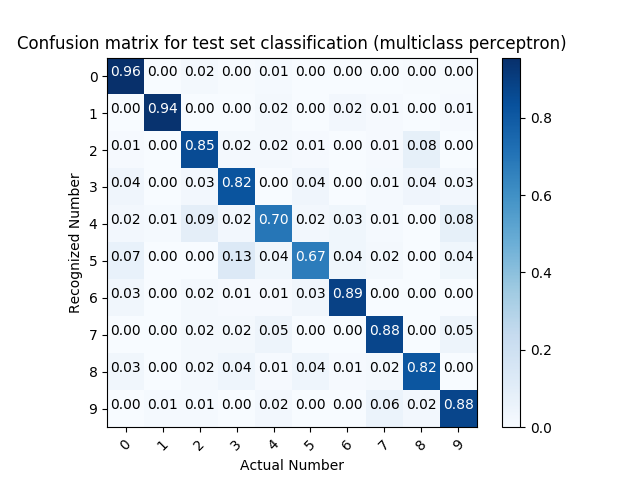
\includegraphics[width=0.9\linewidth]{img/4/cm_multi_class_perceptron.png}
\caption{Confusion matrix for the multiclass perceptron net.}
\label{fig:cmperceptron}
\end{figure}

Overall 863 of 1000 test samples were classified correctly.


\section{Excercise 5: Gradient Descent}
%monitor two values: the MSE made by your network on the training set (it should be dropping), and the number of misclassified inputs.%
%alternative functions tanh, relu%
%using various initialization strategies and values of the learning rate%
In order to monitor the \emph{mean-squared-error} (MSE) for different activation functions, different weight initialization strategies and different learning rates we decided to plot multiple line charts where on the x-axis the amount of iterations and on the y-axis the MSE is portrayed.
We purposely did not include the initial MSE, because it heavily drops after the first iteration.
This is especially true for the \emph{hyperbolic tangent} which sometimes starts at $MSE=100$.

We did the same with the misclassified inputs, but obviously the y-axis displays the number of misclassified inputs this time.

\subsection{Test cases}

We thought about some test cases and decided to test with the following strategies:

\begin{itemize}
\item{Learning rate $\eta = \{0.1\ |\ 0.5\ |\ 1.0\ |\ 2.0\ |\ 4.0 \}$}
\item{Weight initialization strategy: $w = \{ random\ |\ all\ 0.0\ |\ all\ 0.5\ |\ all\ 1.0\}$}
\item{Activation function $\phi = \{sigmoid | linear rectifier | hyberbolic tangent\}$}
\item{2000 iterations}
\end{itemize}


% TODO HYPERBOLIC ACTIVATION FUNCTION IMPLEMENTATION IS WRONG!

\subsection{Evaluation}
We combined all possible combinations to evaluate the best strategy.
To compare the three activation functions, we decided to plot them all together in one chart.
After generating the plots, we looked for the best results for every activation function.
\\

Given the evaluation graphs we can conclude that the \emph{sigmoid} activation function performs best if the learning rate is very high ($\eta = 2$) and the weights are initialized randomly (see Figure \ref{fig:best_result_sigmoid_mse}).  Here we almost reach $MSE = 0$. You can also see the good result in the graph of the misclassified inputs (see Figure \ref{fig:best_result_sigmoid_inputs}. After around 230 iterations the neural network classifies all inputs correctly (with the sigmoid activation function).

\begin{figure}[H]
	\centering
	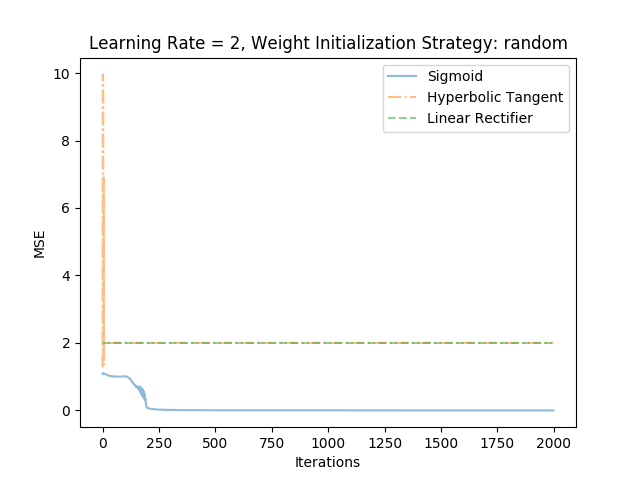
\includegraphics[width=0.9\linewidth]{img/5/sigmoid-mse.png}
	\caption{MSE evolution with all weights initialized randomly and learning rate 2}
	\label{fig:best_result_sigmoid_mse}
\end{figure}

\begin{figure}[H]
	\centering
	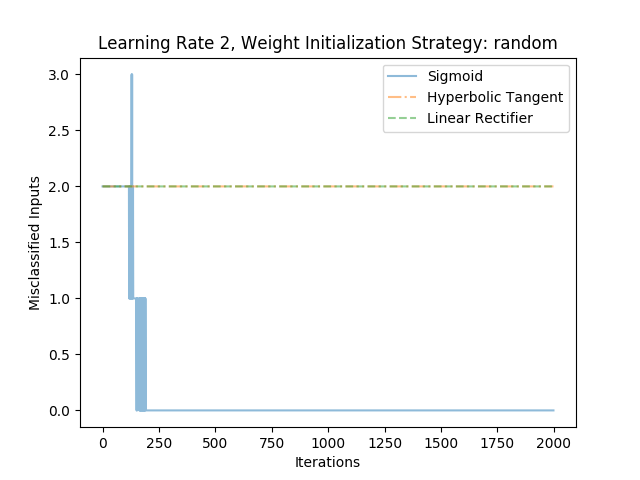
\includegraphics[width=0.9\linewidth]{img/5/sigmoid-inputs.png}
	\caption{Misclassified inputs with all weights initialized randomly and learning rate 2}
	\label{fig:best_result_sigmoid_inputs}
\end{figure}


The \emph{linear rectifier} activation function usually produces very bad results, except if the learning rate is 0.1 and the weights are initialized randomly where it almost reaches $MSE = 0$ (see Figure \ref{fig:best_result_linrect_mse}). After around 400 iterations the neural network classifies all inputs correctly (with the linear rectifier activation function).

\begin{figure}[H]
	\centering
	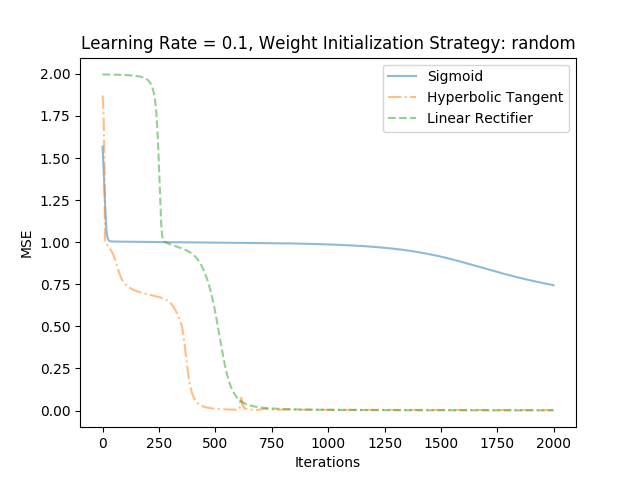
\includegraphics[width=0.9\linewidth]{img/5/linear-rectifier-mse.png}
	\caption{MSE evolution with all weights initialized randomly and learning rate 0.1}
	\label{fig:best_result_linrect_mse}
\end{figure}

\begin{figure}[H]
	\centering
	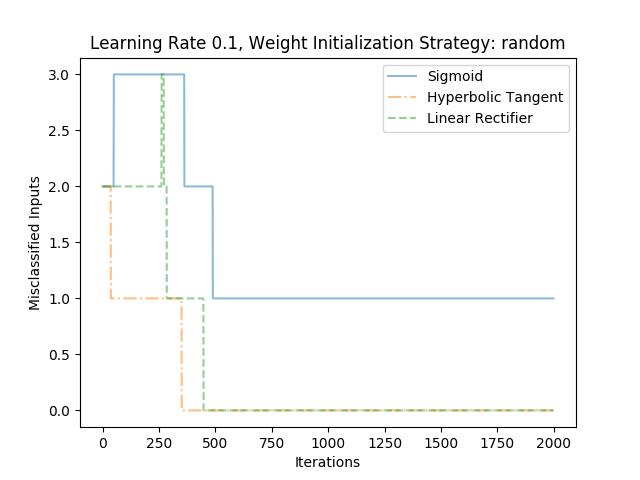
\includegraphics[width=0.9\linewidth]{img/5/linear-rectifier-inputs.png}
	\caption{Misclassified inputs with all weights initialized randomly and learning rate 0.1}
	\label{fig:best_result_linrect_inputs}
\end{figure}


The \emph{hyperbolic tangent} activation function is quite unpredictable. Usually it produces very bad results, or the MSE jitters heavily per iteration (see Figure \ref{fig:tangent-jitter}).
The best stable result we were able to achieve have the same parameters as the best linear rectifier result. The MSE reaches almost 0 after 375 iterations (see Figure \ref{fig:best_result_linrect_mse}). Also after around 375 iterations, all inputs are classified correctly (see Figure \ref{fig:best_result_linrect_inputs}.

\begin{figure}[H]
	\centering
	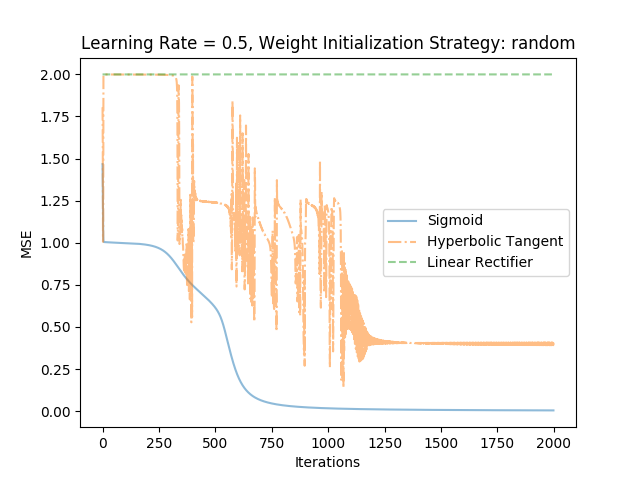
\includegraphics[width=0.9\linewidth]{img/5/tangent-jitter.png}
	\caption{Jitter of the hyperbolic tangent function}
	\label{fig:tangent-jitter}
\end{figure}


\end{document}